\section*{Разработка интерфейса}
\addcontentsline{toc}{section}{Разработка интерфейса}

Для любой программы интерфейс является одной из наиболее важных составляющих.
Ведь именно он определяет, как приложение будет взаимодействовать с другими
программами и своими пользователями. Таким образом, можно ввести следующую
классификацию интерфейсов:

\setlist{nolistsep}
\begin{enumerate}
    \item Программные
    \item Графические
    \item Интерфейсы командной строки
\end{enumerate}

Несмотря на то, что эти интерфейсы имеют между собой мало общего, к ним 
предъявляется ряд общих требований:

\begin{enumerate}
    \item Функциональность -- интерфейс должен отвечать всем требованиям пользователя и соответствовать его задачам;
    \item Логичность -- интерфейс должен быть логичным и запоминающимся, чтобы взаимодействие пользователя
        с программой было как можно более простым и удобным;
    \item Защищенность -- интерфейс должен быть спроектирован таким образом, чтобы у пользователя не было
        возможности совершить ошибку.
\end{enumerate}

После определения общих требований к любому интерфейсу, стоит рассмотреть перечисленные выше
интерфейсы отдельно.

\subsection*{Программные интерфейсы}
\addcontentsline{toc}{subsection}{Программные интерфейсы}

К программным интерфейсам можно причислить любой интерфейс, который предназначен для
использования разрабатываемой программы внешними приложениями. Обычно, в зависимости от
используемых технологий, это набор классов, функций или методов, которые используются
внешними программами. В случае данного приложения в качестве интерфейса взаимодействия
было решено использовать веб-технологии. Это означает, что приложение будет взаимодействовать
с любыми своими пользователями через протокол HTTP.
Таким образом, программный интерфейс приложения будет представлять из себя набор HTTP-методов.

В протоколе HTTP есть несколько видов методов, из которых приложением будут использоваться следующие:

\begin{enumerate}
    \item GET -- это методы, которые запрашивают данные и не предназначенные для их записи.
    \item POST -- это методы, которые используются и для записи данных, и для их получения.
\end{enumerate}

Говоря об HTTP интерфейсах, стоит отметить, что есть несколько различных подходов к проектированию
подобных интерфейсов. Одним из наиболее общепринятых подходов является так называемый REST.
Это можно перевести как Represental State Transfer\cite{REST}. Данная архитектура предлагает
наложить на приложение ряд следующих ограничений:

\begin{enumerate}
    \item Модель клиент-сервер
    \item Отсутствие состояния
    \item Кэширование
    \item Единообразие интерфейса
    \item Слои
\end{enumerate}

Такой подход позволяет добиться лучшей производительности за счет отсутствия состояний между
вызовами и кэширования, а архитектура становится более расширяемой из-за требований
единообразия и использования слоев.

\subsection*{Графические интерфейсы}
\addcontentsline{toc}{subsection}{Графические интерфейсы}

Графические интерфейсы -- это наиболее востребованные интерфейсы в современном мире, потому
что пользователям намного более удобно пользоваться интерфейсами, у которых среди
средств донесения информации есть не только текст. 

И, пожалуй, самый популярный вид графических приложений -- это веб-сайты.
Они получили такую популярность из-за своей универсальности: пользователь
может открыть приложение на любом устройстве, на котором есть доступ в интернет
и веб-браузер, в то время как любое другое приложение потребует установки
на устройство пользователя.

//Продолжить, если/когда дело дойдет до написания

\subsection*{Интерфейсы командной строки}
\addcontentsline{toc}{subsection}{Интерфейсы командной строки}

Интерфейсы командной строки, в отличии от графических и программных интерфейсов, представляют
наименее популярную группу приложений. Но, несмотря на это, они являются
незаменимыми. Главное преимущество приложений командной строки заключается в том, что
ими могут пользоваться в равной степени эффективно человек, и программа. Таким образом,
интерфейсы командной строки являются сочетанием программных и графических интерфейсов:
с одной стороны ими с определенной степенью удобства может пользоваться человек, а с другой
стороны без каких-либо трудностей они могут использоваться для взаимодействия между
приложениями. Также стоит отметить, что приложениям командной строки не нужен какой-либо
графический интерфейс, только окно терминала.

Для того, чтобы заниматься непосредственным проектированием интерфейсов, необходимо
понять задачу, которые они будут решать.

\subsection*{Постановка задачи}
\addcontentsline{toc}{subsection}{Постановка задачи}

Необходимо разработать приложение, которое выполняет генерацию списков литературы
для учебных курсов в формате BibTeX. Для этого приложение должно иметь следующие функции:

\begin{enumerate}
    \item Поиск информации о книгах;
    \item Хранение и модификация информации о книгах;
    \item Создание и модификация данных об учебных курсах;
    \item Генерация списка литературы.
\end{enumerate}

\subsection*{Разработка программного интерфейса}
\addcontentsline{toc}{subsection}{Разработка программного интерфейса}

При рассмотрении программных интерфейсов была описана архитертура REST. Согласно
этой архитектуре каждый метод должен принимать в себя всю необходимую информацию
для выполнения запроса, а все методы должны быть унифицированы. Таким образом, для каждого
вида данных был реализован следующий набор методов:

\begin{itemize}
    \item add\%Вид данных\% -- POST запрос, содержащий данные для добавления в теле.
    \item get\%Вид данных\% -- GET запрос, запрашивающий данные от приложения
    \item modify\%Вид данных\% -- // Более подробно после реализации
    \item delete\%Вид данных\% -- // Более подробно после реализации
\end{itemize}

//Описать дополнительные команды вроде migrate и generate;

\subsection*{Разработка интерфейса командной строки}
\addcontentsline{toc}{subsection}{Разработка интерфейса командной строки}

Как уже было сказано выше, для интерфейсов командной строки крайне важна автоматизируемость.
Это делает невозможным использование так называемого интерактивного ввода. Другими словами,
любое действие пользователя должно совершаться за один вызов приложения. В результате
было решено использовать следующий подход к проектированию интерфейса: для каждого вида данных,
с которыми будет работать приложение, будет реализован следующих набор методов:

\begin{itemize}
    \item get\%Вид данных\%Prototype -- данный метод добавляет новый файл в файловую систему,
        который содержит в себе прототип для нужного вида данных. После чего пользователь
        должен заполнить этот прототип информацией, которую хочет добавить;
    \item add\%Вид данных\% -- сохраняет данные в приложение;
    \item get\%Вид данных\% -- позволяет получить данные из приложения, можно конфигурировать
        флагами;
    \item modify\%Вид данных\% -- позволяет модифицировать данные в приложении; // Более подробно после реализации
    \item delete\%Вид данных\% -- позволяет удалять данные в приложении; // Более подробно после реализации
\end{itemize}

Также отличительной чертой хорошего приложения командной строки является грамотно оформленная справка.
Рисунок 1 показывает результат выполнения команды help. 

\begin{figure}[h]
    \center{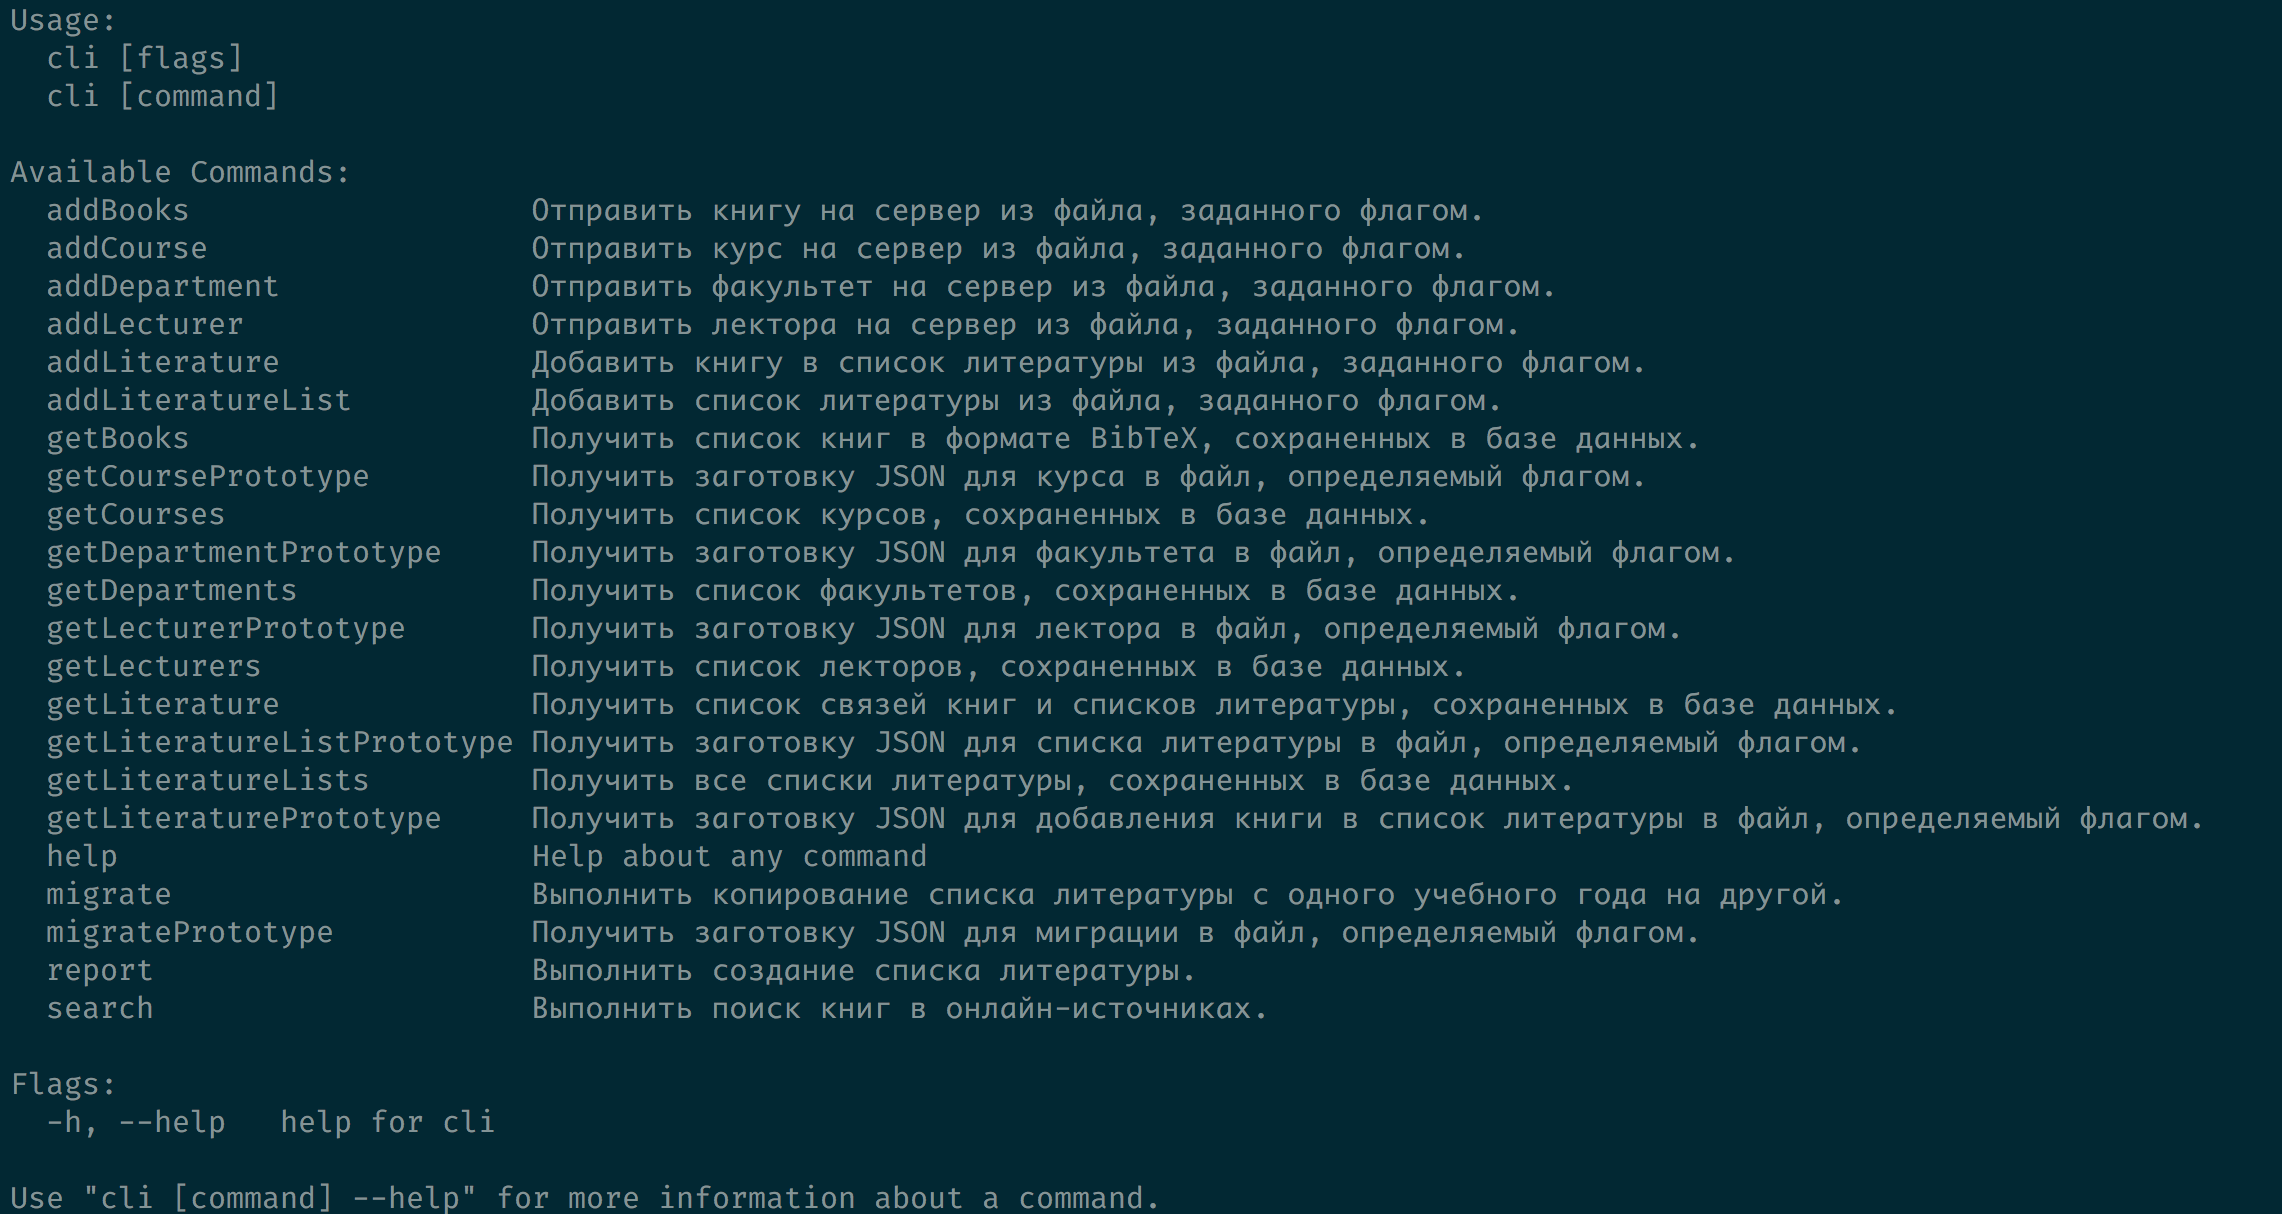
\includegraphics[width=1\linewidth]{help}}
    \caption{Пример работы команды help.}
    \label{ris:image}
\end{figure}

Также для каждой отдельной команды реализован
отдельный флаг --help, который показывает справку для конкретной команды, что можно видеть на рисунке 2. 

\begin{figure}[h]
\center{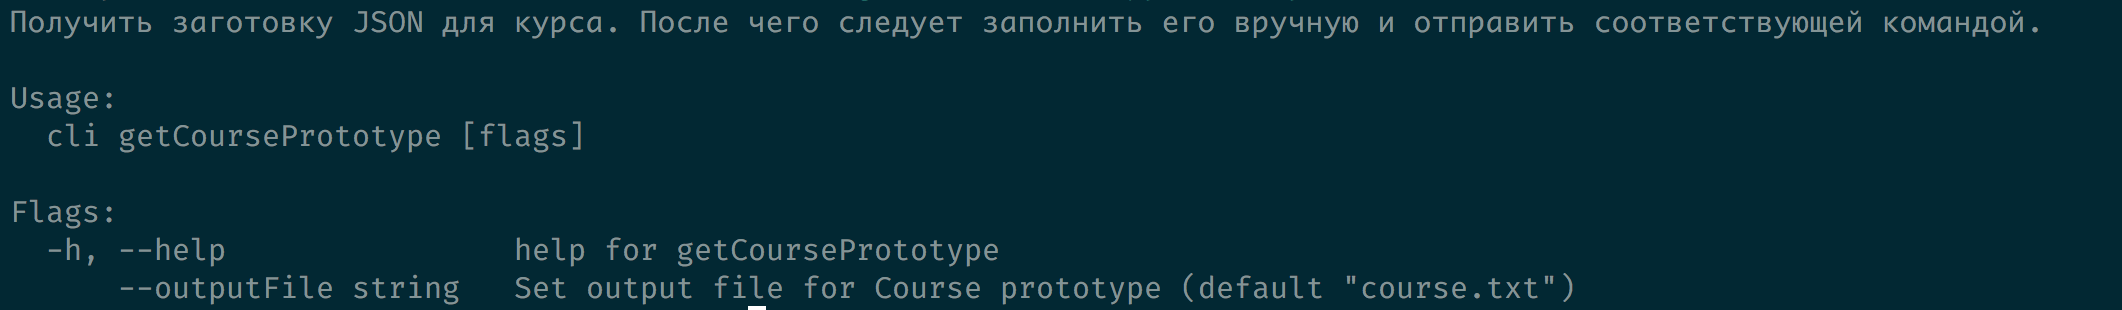
\includegraphics[width=1\linewidth]{help_get_course_prototype}}
\caption{Пример работы флага --help для команды getCoursePrototype.}
\label{ris:image}
\end{figure}


//Описать дополнительные команды вроде migrate и generate; сделать скриншоты работы программы

\subsection*{Разработка графического интерфейса}
\addcontentsline{toc}{subsection}{Разработка графического интерфейса}

//Написать, если/когда дело дойдет до написания